\section{Q2: Overhead}
\label{sec:perf}

\paragraph{Method.} Benchmarks are built at \code{-O2 -g -fno-omit-frame-pointer}. ASan adds
\code{-fsanitize=address}, and Valgrind runs the uninstrumented binary. Each configuration runs five
times. SQLite and Lua wall times and all peak resident set sizes (RSS) come from
\code{/usr/bin/time}; the allocator micro-benchmark records its workload time with a monotonic clock.
We report five-run medians and ratios against the uninstrumented baseline of the same configuration.
Valgrind's RSS includes the tool's own memory. There are three workloads. The first is SQLite~3.50.4
\code{speedtest1}~\cite{sqlitespeedtest} (\code{-{}-memdb -{}-size 100 -{}-testset main}) in SQLite's
default configuration and with memsys5 serving all allocations from a 256~MiB heap (minimum block 64
bytes). The second is a synthetic Lua~5.4.9 workload~\cite{lua} that builds, sorts and garbage-collects
20 rounds of 100{,}000 tables with strings, with Lua's stock allocator. The third is an allocator
micro-benchmark that runs 10{,}000 allocation and reuse cycles on Arena and Free list with annotation
off and on, and on their rewrites. The first two ran on the VirtualBox VM and the third on EC2
(Table~\ref{tab:env}), and numbers are compared only within one machine. HWASan was not measured, because its only host is a
laptop VM whose timings cannot be compared with the others.

\begin{table}[t]
\centering\small
\begin{tabular}{llrrrr}
\toprule
workload & tool & time (s) & $\times$ & peak RSS (MiB) & $\times$ \\
\midrule
SQLite speedtest1, default & baseline & \shortstack{2.30\\{\scriptsize[2.24, 2.46]}} & 1.00 & \shortstack{77.1\\{\scriptsize[77.0, 77.1]}} & 1.00 \\[3pt]
 & ASan & \shortstack{6.08\\{\scriptsize[5.97, 6.50]}} & 2.64 & \shortstack{611.4\\{\scriptsize[590.1, 611.6]}} & 7.94 \\[3pt]
 & Memcheck & \shortstack{62.04\\{\scriptsize[60.46, 63.17]}} & 26.97 & \shortstack{189.7\\{\scriptsize[189.6, 189.7]}} & 2.46 \\[3pt]
\addlinespace
SQLite speedtest1, memsys5 & baseline & \shortstack{2.47\\{\scriptsize[2.33, 2.69]}} & 1.00 & \shortstack{121.2\\{\scriptsize[121.0, 121.3]}} & 1.00 \\[3pt]
 & ASan & \shortstack{5.34\\{\scriptsize[5.07, 5.58]}} & 2.16 & \shortstack{166.5\\{\scriptsize[166.4, 166.7]}} & 1.37 \\[3pt]
 & Memcheck & \shortstack{60.58\\{\scriptsize[59.31, 61.31]}} & 24.53 & \shortstack{208.3\\{\scriptsize[208.3, 208.4]}} & 1.72 \\[3pt]
\addlinespace
Lua 5.4.9 table/GC workload & baseline & \shortstack{4.65\\{\scriptsize[4.30, 4.75]}} & 1.00 & \shortstack{29.7\\{\scriptsize[29.6, 29.7]}} & 1.00 \\[3pt]
 & ASan & \shortstack{13.85\\{\scriptsize[13.25, 15.06]}} & 2.98 & \shortstack{473.4\\{\scriptsize[473.3, 474.0]}} & 15.94 \\[3pt]
 & Memcheck & \shortstack{133.64\\{\scriptsize[130.16, 134.60]}} & 28.74 & \shortstack{188.4\\{\scriptsize[188.3, 188.6]}} & 6.34 \\[3pt]
\bottomrule
\end{tabular}

\caption{Tool overhead on real programs (VirtualBox VM, median of five runs, $\times$ = ratio to the
baseline of the same configuration). No custom annotations.}
\label{tab:perf-tools}
\end{table}

\begin{figure}[t]
\centering
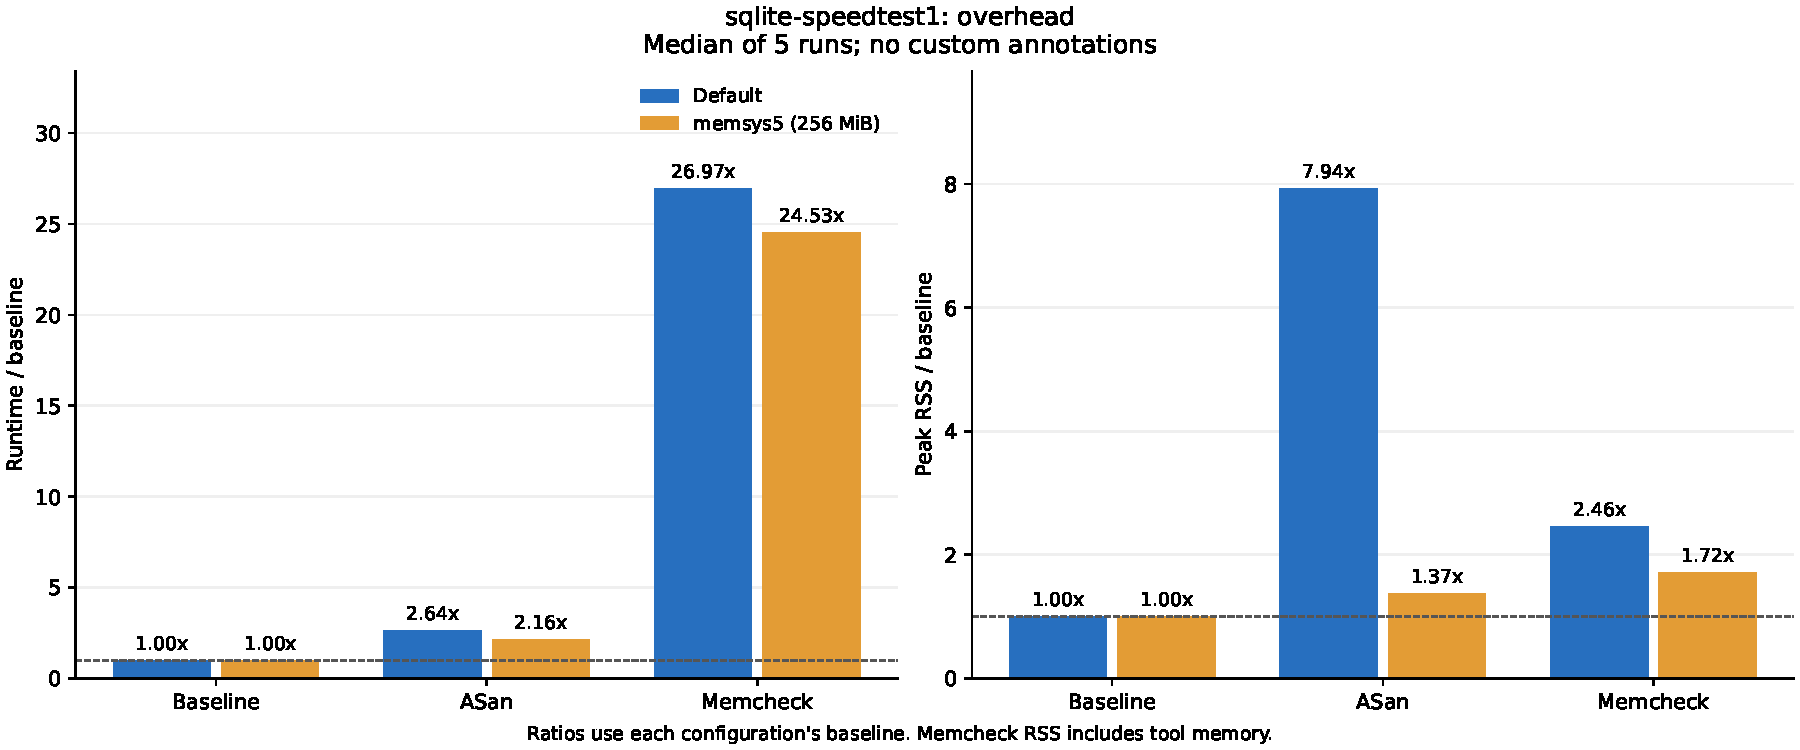
\includegraphics[width=0.92\textwidth]{figures/benchmark-overhead.pdf}
\caption{SQLite \code{speedtest1} overhead in time and peak RSS, default allocator versus memsys5.}
\label{fig:speedtest}
\end{figure}

\paragraph{Tool overhead.} Table~\ref{tab:perf-tools} and Figure~\ref{fig:speedtest} show the
familiar picture: ASan costs 2.2--3.0$\times$ in time, Valgrind 24.5--28.7$\times$. Memory is where
the allocator matters. With SQLite's default allocator ASan's peak RSS is 7.9$\times$ the baseline
(611~MiB). With memsys5 it is 1.4$\times$ (167~MiB), and its time overhead also drops, from
2.64$\times$ to 2.16$\times$. On Lua, which allocates many small objects through the stock allocator,
ASan's RSS reaches 15.9$\times$. The likely reason is the one behind Q1: ASan pays redzones and
quarantine per \code{malloc} block, and under memsys5 there is a single 256~MiB block, so SQLite's
objects carry no redzones and their frees enter no quarantine. The lower overhead is the price of
the lost visibility measured in \S\ref{sec:q1-blind} --- a sanitizer run that is cheaper under a CMA
is also checking less. Valgrind's overhead is dominated by binary translation and changes little.

\begin{table}[t]
\centering\small
\begin{tabular}{llrrrrr}
\toprule
allocator & tool & off (s) & on (s) & on/off & RSS off / on (MiB) & rewrite (s, MiB) \\
\midrule
Arena & ASan & \shortstack{1.510\\{\scriptsize[1.466, 2.130]}} & \shortstack{1.582\\{\scriptsize[1.572, 1.820]}} & 1.05$\times$ & 46.1 / 46.0 & 0.547, 154 \\[3pt]
 & Memcheck & \shortstack{2.273\\{\scriptsize[2.268, 2.281]}} & \shortstack{4.038\\{\scriptsize[4.034, 4.138]}} & 1.78$\times$ & 72.0 / 72.3 & 2.672, 142 \\[3pt]
Free list & ASan & \shortstack{1.478\\{\scriptsize[1.463, 2.488]}} & \shortstack{1.625\\{\scriptsize[1.617, 1.625]}} & 1.10$\times$ & 43.6 / 43.6 & 0.535, 154 \\[3pt]
 & Memcheck & \shortstack{2.413\\{\scriptsize[2.405, 2.445]}} & \shortstack{5.209\\{\scriptsize[5.197, 5.252]}} & 2.16$\times$ & 72.9 / 72.8 & 2.686, 142 \\[3pt]
\bottomrule
\end{tabular}

\caption{Annotation overhead on the allocator micro-benchmark (EC2, median of five runs). ``off'' and
``on'' are the plain and annotated builds of the same allocator, and the last column is the rewrite.}
\label{tab:perf-churn}
\end{table}

\paragraph{Annotation overhead.} On the allocation-heavy loop (Table~\ref{tab:perf-churn},
Figure~\ref{fig:churn}), ASan's annotations add 5--10\%: poisoning and unpoisoning a region are plain
shadow-memory writes. Memcheck's annotations cost
1.78$\times$ on Arena and 2.16$\times$ on Free list, because every pool request is a client request
that Memcheck must process and record. The Free list issues more of them, since it also opens and
closes its in-slot link. Annotation does not change peak RSS for either tool. The rewrites are faster
under ASan (0.54~s against 1.5~s) but use 3.3$\times$ as much memory (154~MiB against 46~MiB), the
per-object redzones and quarantine that make them detectable. They change the allocation algorithm
and lifetimes, so their numbers are a different trade-off, not an annotation cost.

\begin{figure}[t]
\centering
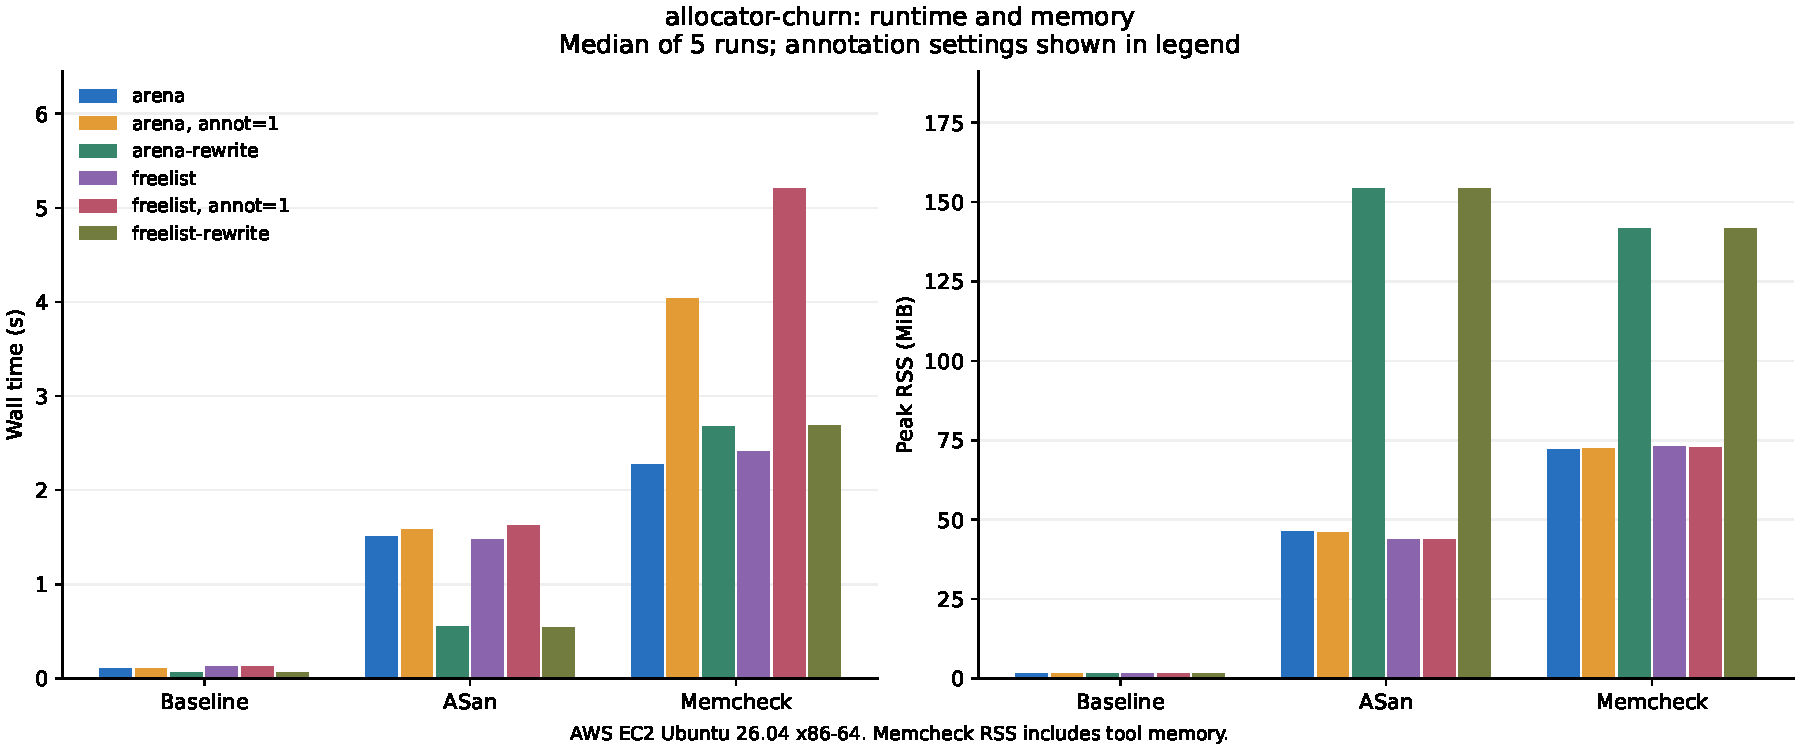
\includegraphics[width=0.92\textwidth]{figures/part-b-churn-performance.pdf}
\caption{Allocator micro-benchmark on EC2: wall time and peak RSS per allocator, annotation setting
and tool.}
\label{fig:churn}
\end{figure}

For a project deciding how to test a program with a CMA, the two questions meet here. Annotating for
ASan is nearly free and recovers most bugs. Annotating for Memcheck roughly doubles an already large
cost but also catches bad frees. A rewrite gives \code{malloc}-level detection at \code{malloc}-level
memory cost, while giving up whatever behaviour the CMA provided.
